\documentclass[ngerman]{beamer}
\usepackage{babel}
\usepackage[latin1]{inputenc}
\usepackage[T1]{fontenc}
\usepackage{lmodern}
\usepackage{graphicx}

    \usetheme{TUC2}
%    \usefonttheme{structureitalicserif}
    \setbeamercovered{transparent}

\mode<presentation>
    \title{Amazon EC2}
    \subtitle{EC2 virtual server und EC2 container}
    \author{Christian Rebischke}
    \institute{Institut f�r Informatik}
    \date{2017-07-04}


%%%%%%%%%%%%%%%%%%%%%%%%%%%%%%%%%%%%%%%%%%%%%%%%%%%%%%
\begin{document}
\begin{frame}
\titlepage
\end{frame}

\begin{frame}
\frametitle{Agenda}
\tableofcontents
\end{frame}
%%%%%%%%%%%%%%%%%%%%%%%%%%%%%%%%%%%%%%%%%%%%%%%%%%%%%%

\section{Einf�hrung in Amazon EC2}
\begin{frame}
    \frametitle{Warum Amazon EC2?}
    \begin{itemize}
        \item Flexible Kosten
        \item Weltweite Infrastruktur
        \item Software as a Service
        \item Einfache Skalierung
        \item Server on Demand
    \end{itemize}
\end{frame}

\begin{frame}
    \frametitle{Vertikale vs Horizontale Skalierung}
    \includegraphics[width=0.8\textwidth]{figures/scalability.pdf}
\end{frame}

\begin{frame}
    \frametitle{Begrifflichkeiten}
    \begin{itemize}
        \item Amazon Machine Image (AMI)
        \item Instance Type
    \end{itemize}
    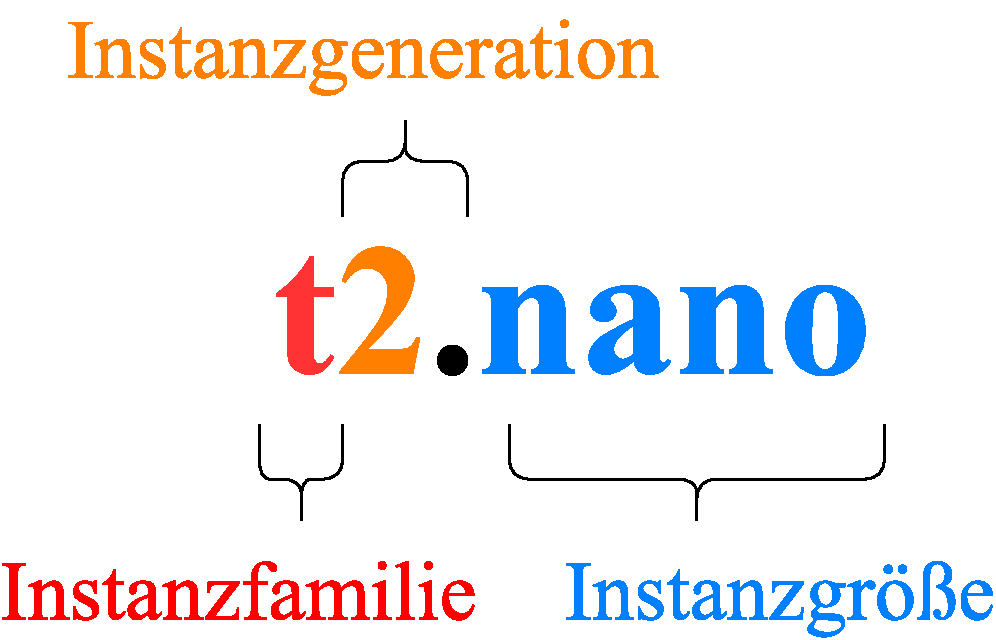
\includegraphics[width=0.5\textwidth]{figures/instance.pdf}
\end{frame}

\begin{frame}
    \frametitle{Die EC2 Landschaft}
    \includegraphics[width=0.7\textwidth]{figures/EC2-Landscape.pdf}
\end{frame}

\section{Regionen}
\begin{frame}
    \frametitle{Verteilte Infrastruktur}
    \begin{itemize}
        \item Rechenzentren �ber die Welt verstreut
            \begin{itemize}
                \item USA
                \item Deutschland
                \item \dots
            \end{itemize}
        \item Pro Land mehrere High-Availability-Zonen
        \item Beispielsweise USA-West-1 (Ohio)
    \end{itemize}
\end{frame}

\section{Virtualisierungstechnik}
\begin{frame}
    \frametitle{Was ist Virtualisierung?}
    \begin{itemize}
        \item Nachbildung von Hardware oder Software-Schnittstellen
        \item Abstraktionsschicht
        \item Ausf�hren eines Betriebssystems in einem anderen
        \item Aufteilung von System-Ressourcen
    \end{itemize}
\end{frame}

\begin{frame}
    \frametitle{Visualisierung der Hypervisor Technologie}
    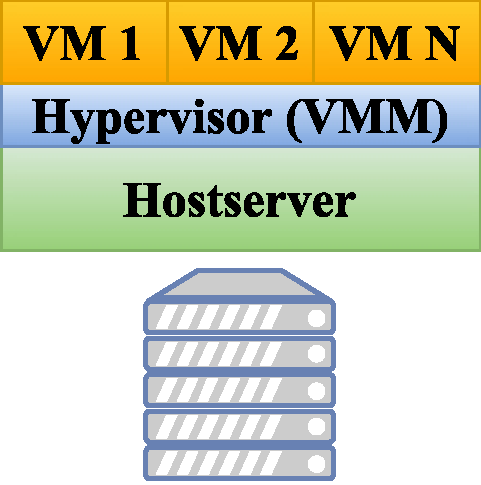
\includegraphics[width=0.5\textwidth]{figures/hypervisor.pdf}
\end{frame}

\begin{frame}
    \frametitle{Amazons Virtualisierungstechnologien}
    \begin{itemize}
        \item PV
            \begin{itemize}
                \item steht f�r paravirtual
                \item hat einen speziellen Bootloader
                \item Virtualisierung nur durch Software
                \item Kein Zugriff auf Hardware-Schnittstellen
            \end{itemize}
        \item HVM
            \begin{itemize}
                \item steht f�r hardware virtual machine
                \item performanter
                \item echte virtualisierung auf Hardware-Ebene
                \item Zugriff auf Hardware-Schnittstellen
            \end{itemize}
    \end{itemize}
\end{frame}

\begin{frame}
    \frametitle{PV und HVM im Vergleich}
    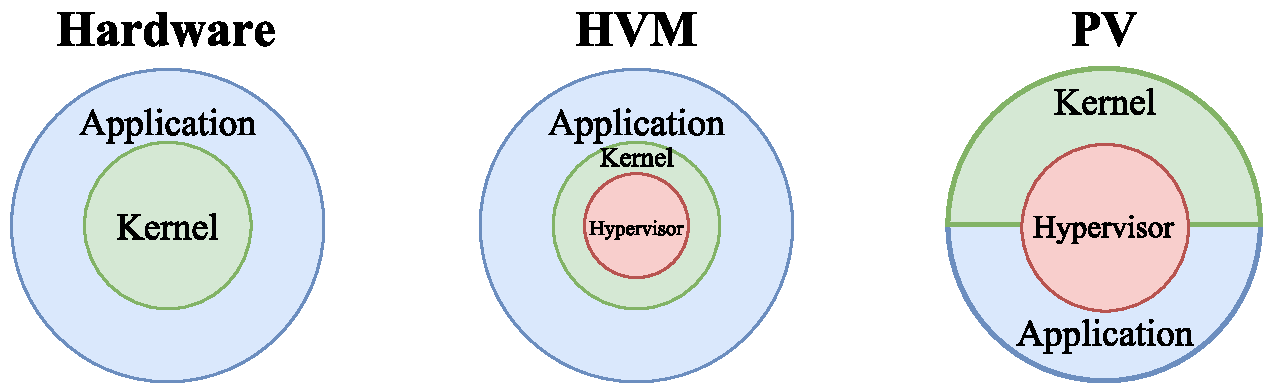
\includegraphics[width=1.0\textwidth]{figures/hvm_pv.pdf}
\end{frame}

\section{EC2 Container}
\begin{frame}
    \frametitle{Was sind Container?}
    \begin{itemize}
        \item keine Virtualisierung
        \item Isolation
        \item Betriebssystem-Kernel Support ben�tigt
        \item Isolation von Applikationen oder ganzen Betriebssystemen
        \item Bekannte Technologien: Docker, LXC, systemd-nspawn
    \end{itemize}
\end{frame}

\begin{frame}
    \frametitle{Wie funktionieren Container}
    \begin{itemize}
        \item namespace
        \item cgroups
        \item Union File Systems
    \end{itemize}
\end{frame}

\begin{frame}
    \frametitle{Namespace}
    \begin{itemize}
        \item Prozess-Virtualisierung
        \item setns-syscall im Kernel
        \item Verf�gbare Namespaces:
            \begin{itemize}
                \item ipc (Interprozesskommunikation)
                \item net (Netzwerk)
                \item pid (Prozess-Virtualisierung)
                \item mnt (Mount-Points/Andockstellen im Filesystem)
                \item uts (Unix-Time-Sharing)
            \end{itemize}
    \end{itemize}
\end{frame}

\begin{frame}
    \frametitle{Cgroups}
    \begin{itemize}
        \item Control Groups
        \item isolieren System-Ressourcen
        \item Gruppiert virtuelle Prozesse
    \end{itemize}
\end{frame}

\begin{frame}
    \frametitle{Union File Systems}
    \begin{itemize}
        \item Abstraktionsschicht im Filesystem
        \item Features wie CoW (Copy-on-Write)
        \item Bekannte Filesysteme: AUFS, btrfs, UnionFS, zfs, xfs
    \end{itemize}
\end{frame}

\begin{frame}
    \frametitle{Amazon EC2 Container}
    \begin{itemize}
        \item Container basierter Cluster 
        \item Als Basis Docker
        \item Effizienter Einsatz von Ressourcen
        \item Webinterface
        \item Integration in andere AWS Dienste
        \item Sehr skalierbar
    \end{itemize}
\end{frame}

\section{Sicherheit}
\begin{frame}
    \frametitle{Sicherheit in Amazon EC2}
    \begin{itemize}
        \item Multi-Faktor-Authentifizierung
        \item Amazon Identity and Access Management (IAM)
        \item Security Groups
    \end{itemize}
\end{frame}

\begin{frame}
    \frametitle{Traditionelle Firewall}
    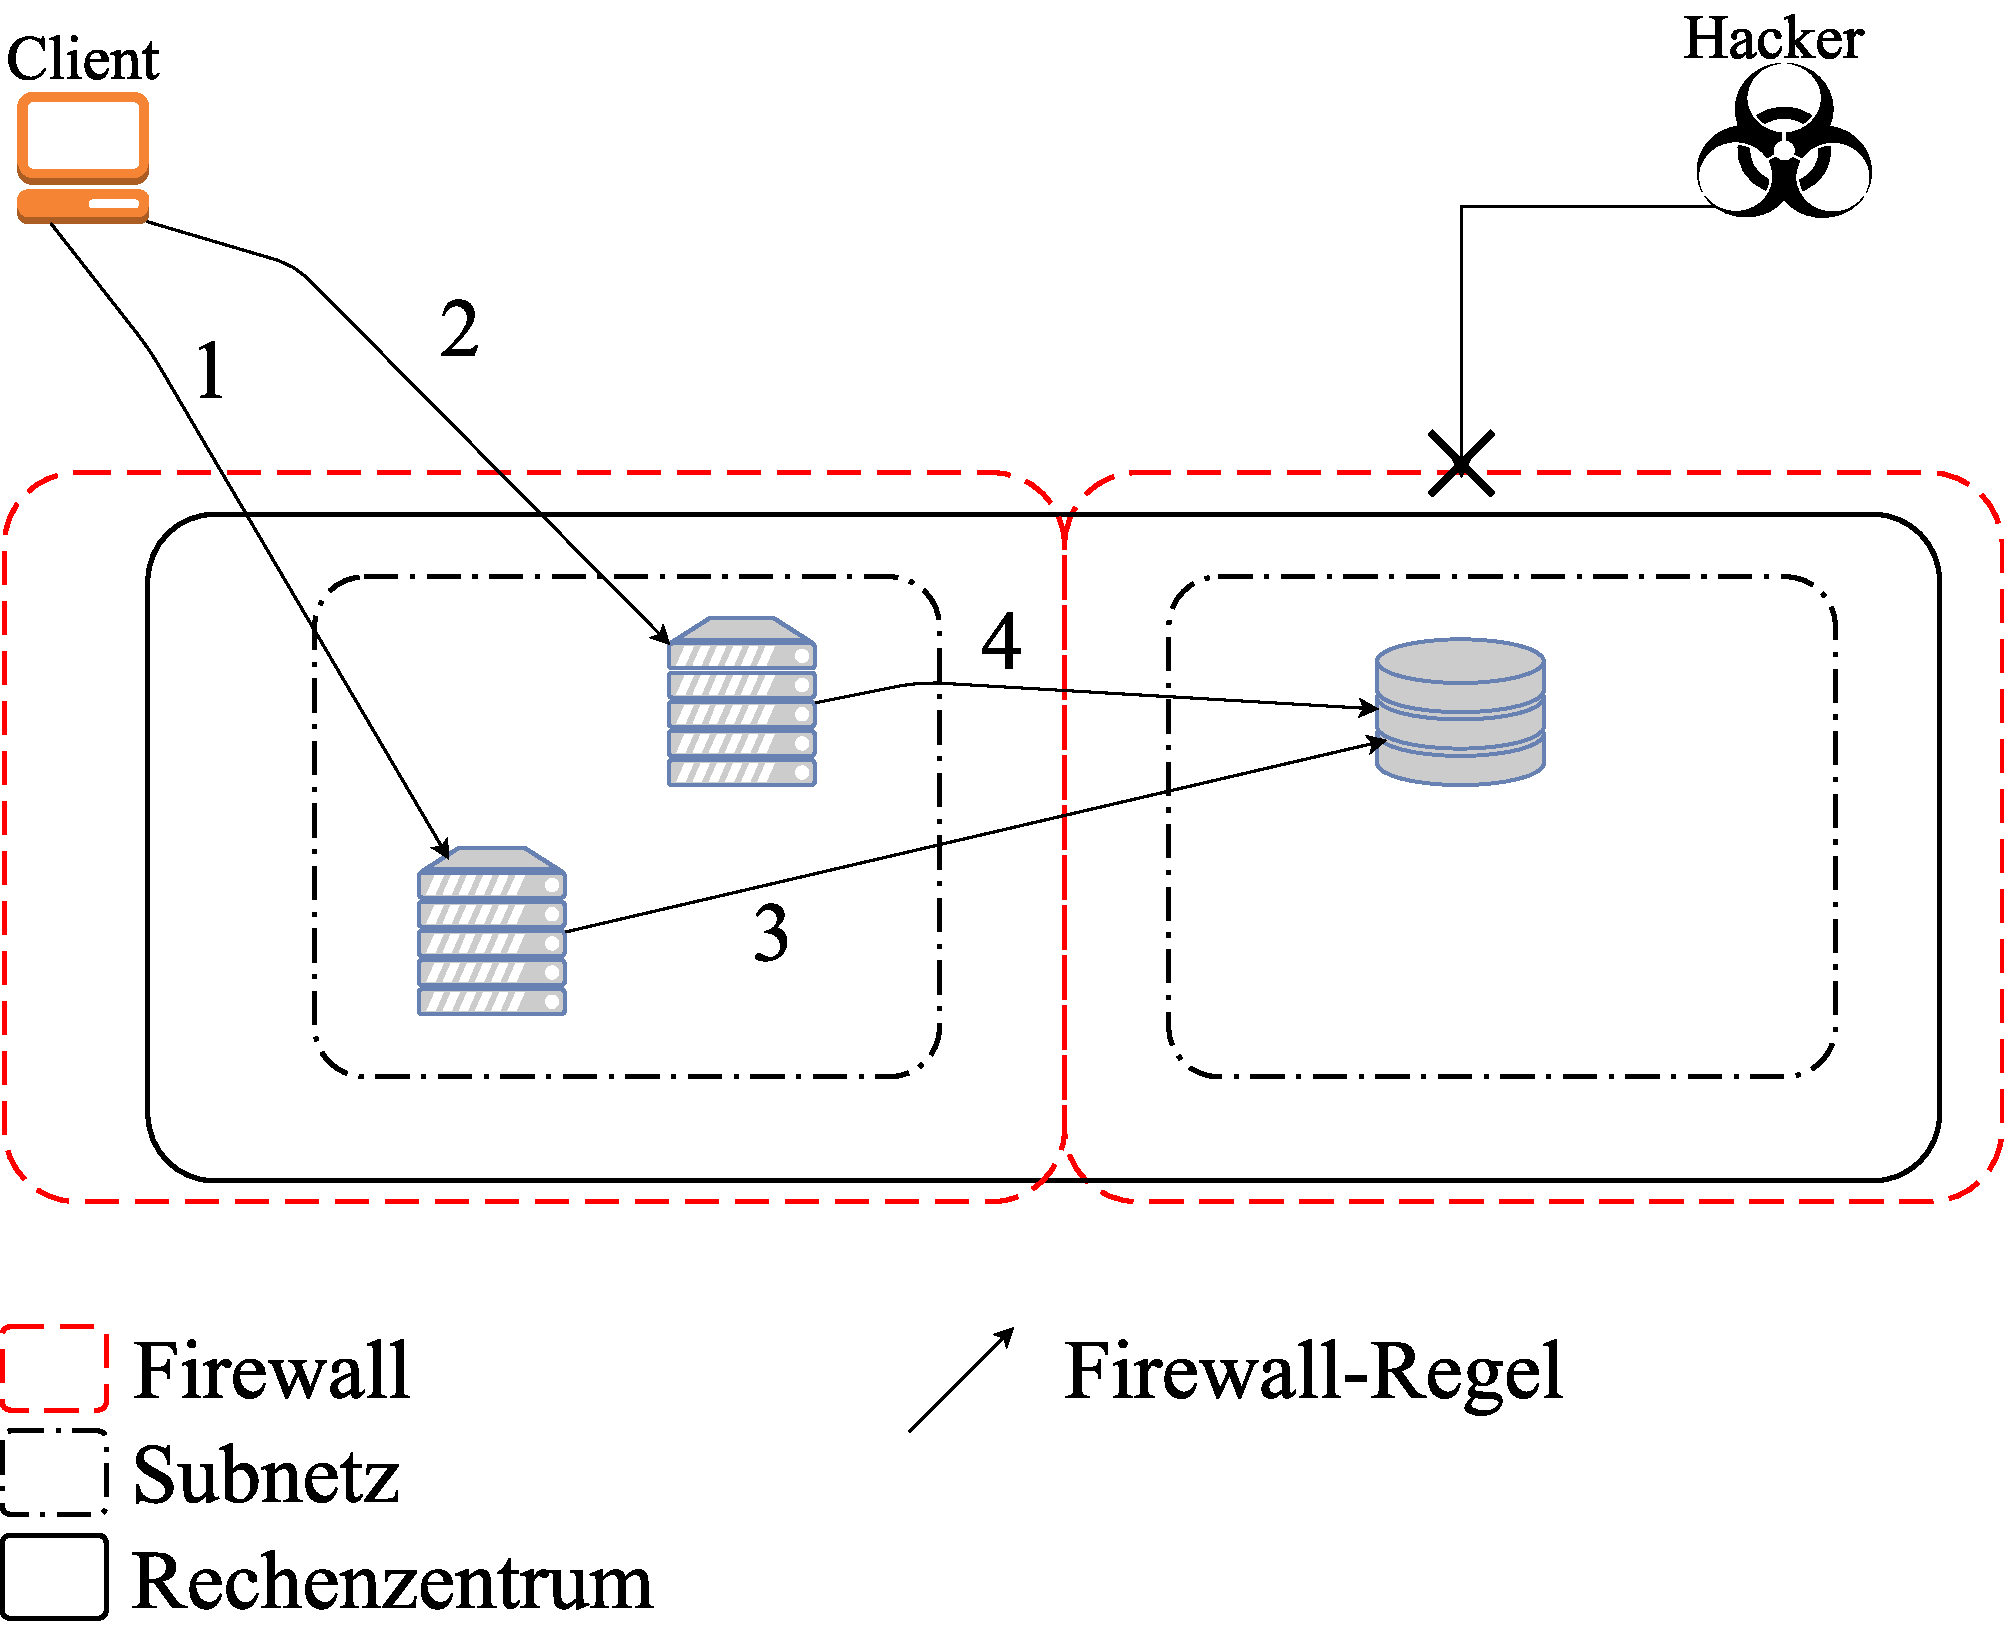
\includegraphics[width=0.7\textwidth]{figures/traditional_firewall.pdf}
\end{frame}

\begin{frame}
    \frametitle{AWS Security Groups}
    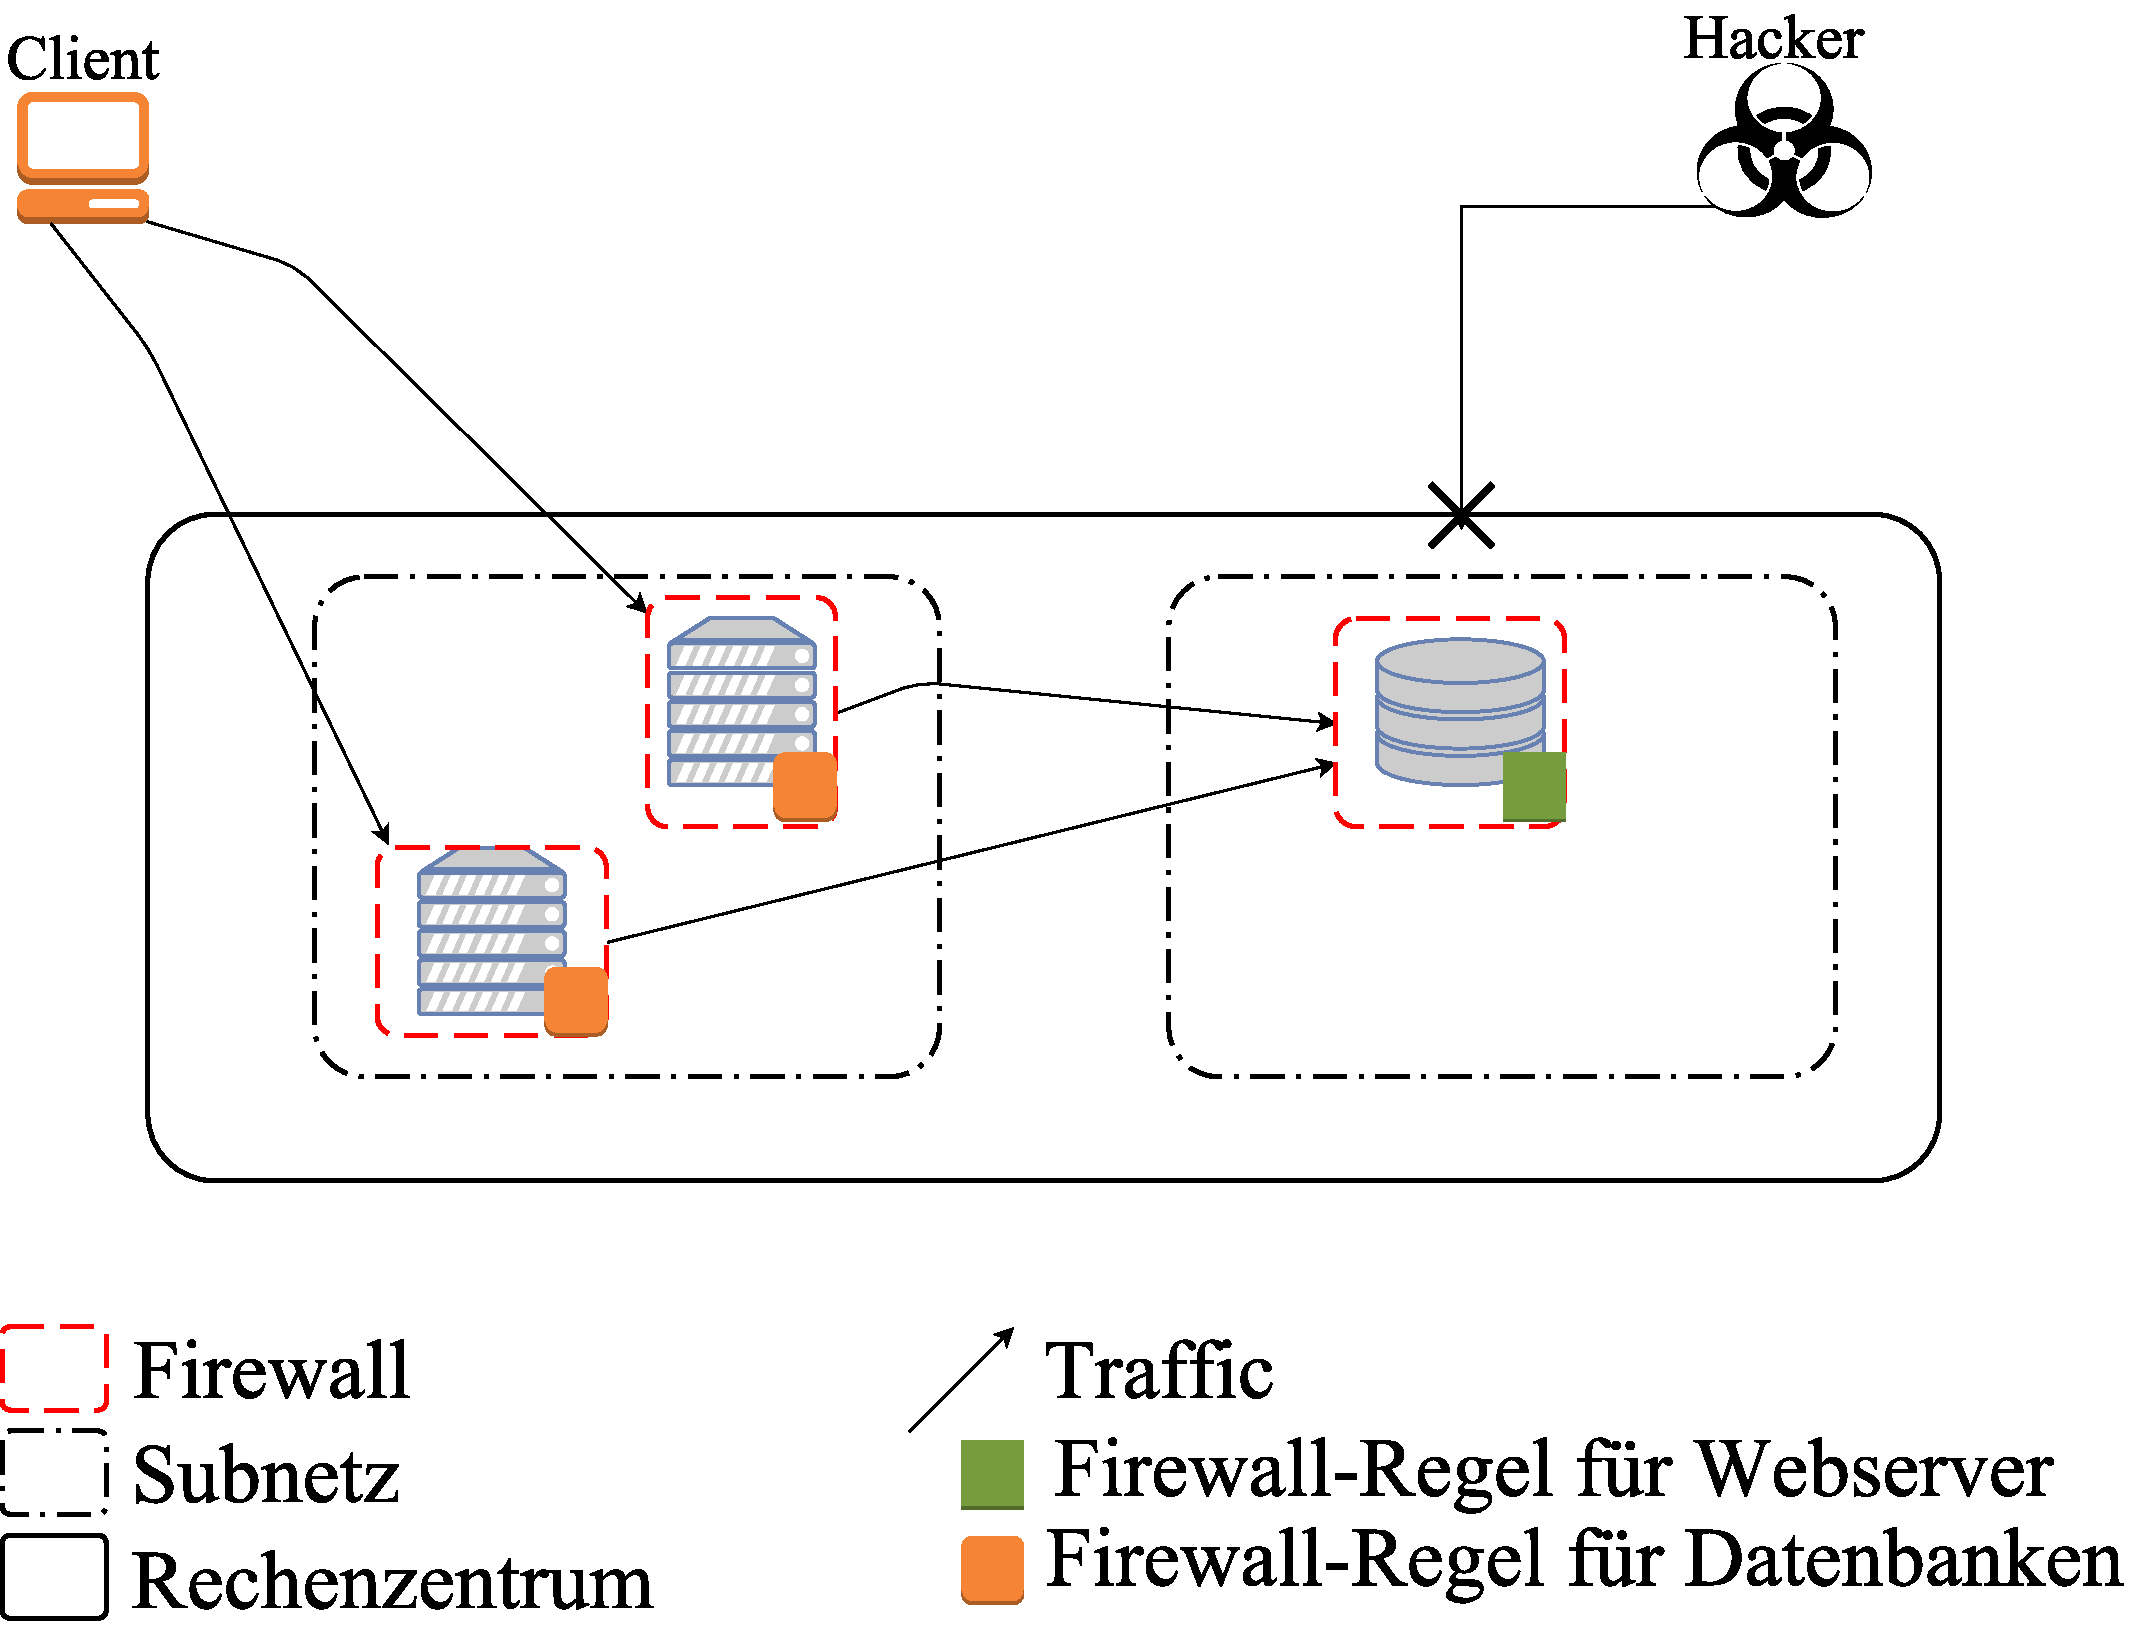
\includegraphics[width=0.7\textwidth]{figures/aws_firewall.pdf}
\end{frame}

\begin{frame}
    \frametitle{Fragen}
\end{frame}

\end{document}
